\documentclass[1p]{elsarticle_modified}
%\bibliographystyle{elsarticle-num}

%\usepackage[colorlinks]{hyperref}
%\usepackage{abbrmath_seonhwa} %\Abb, \Ascr, \Acal ,\Abf, \Afrak
\usepackage{amsfonts}
\usepackage{amssymb}
\usepackage{amsmath}
\usepackage{amsthm}
\usepackage{scalefnt}
\usepackage{amsbsy}
\usepackage{kotex}
\usepackage{caption}
\usepackage{subfig}
\usepackage{color}
\usepackage{graphicx}
\usepackage{xcolor} %% white, black, red, green, blue, cyan, magenta, yellow
\usepackage{float}
\usepackage{setspace}
\usepackage{hyperref}

\usepackage{tikz}
\usetikzlibrary{arrows}

\usepackage{multirow}
\usepackage{array} % fixed length table
\usepackage{hhline}

%%%%%%%%%%%%%%%%%%%%%
\makeatletter
\renewcommand*\env@matrix[1][\arraystretch]{%
	\edef\arraystretch{#1}%
	\hskip -\arraycolsep
	\let\@ifnextchar\new@ifnextchar
	\array{*\c@MaxMatrixCols c}}
\makeatother %https://tex.stackexchange.com/questions/14071/how-can-i-increase-the-line-spacing-in-a-matrix
%%%%%%%%%%%%%%%

\usepackage[normalem]{ulem}

\newcommand{\msout}[1]{\ifmmode\text{\sout{\ensuremath{#1}}}\else\sout{#1}\fi}
%SOURCE: \msout is \stkout macro in https://tex.stackexchange.com/questions/20609/strikeout-in-math-mode

\newcommand{\cancel}[1]{
	\ifmmode
	{\color{red}\msout{#1}}
	\else
	{\color{red}\sout{#1}}
	\fi
}

\newcommand{\add}[1]{
	{\color{blue}\uwave{#1}}
}

\newcommand{\replace}[2]{
	\ifmmode
	{\color{red}\msout{#1}}{\color{blue}\uwave{#2}}
	\else
	{\color{red}\sout{#1}}{\color{blue}\uwave{#2}}
	\fi
}

\newcommand{\Sol}{\mathcal{S}} %segment
\newcommand{\D}{D} %diagram
\newcommand{\A}{\mathcal{A}} %arc


%%%%%%%%%%%%%%%%%%%%%%%%%%%%%5 test

\def\sl{\operatorname{\textup{SL}}(2,\Cbb)}
\def\psl{\operatorname{\textup{PSL}}(2,\Cbb)}
\def\quan{\mkern 1mu \triangleright \mkern 1mu}

\theoremstyle{definition}
\newtheorem{thm}{Theorem}[section]
\newtheorem{prop}[thm]{Proposition}
\newtheorem{lem}[thm]{Lemma}
\newtheorem{ques}[thm]{Question}
\newtheorem{cor}[thm]{Corollary}
\newtheorem{defn}[thm]{Definition}
\newtheorem{exam}[thm]{Example}
\newtheorem{rmk}[thm]{Remark}
\newtheorem{alg}[thm]{Algorithm}

\newcommand{\I}{\sqrt{-1}}
\begin{document}

%\begin{frontmatter}
%
%\title{Boundary parabolic representations of knots up to 8 crossings}
%
%%% Group authors per affiliation:
%\author{Yunhi Cho} 
%\address{Department of Mathematics, University of Seoul, Seoul, Korea}
%\ead{yhcho@uos.ac.kr}
%
%
%\author{Seonhwa Kim} %\fnref{s_kim}}
%\address{Center for Geometry and Physics, Institute for Basic Science, Pohang, 37673, Korea}
%\ead{ryeona17@ibs.re.kr}
%
%\author{Hyuk Kim}
%\address{Department of Mathematical Sciences, Seoul National University, Seoul 08826, Korea}
%\ead{hyukkim@snu.ac.kr}
%
%\author{Seokbeom Yoon}
%\address{Department of Mathematical Sciences, Seoul National University, Seoul, 08826,  Korea}
%\ead{sbyoon15@snu.ac.kr}
%
%\begin{abstract}
%We find all boundary parabolic representation of knots up to 8 crossings.
%
%\end{abstract}
%\begin{keyword}
%    \MSC[2010] 57M25 
%\end{keyword}
%
%\end{frontmatter}

%\linenumbers
%\tableofcontents
%
\newcommand\colored[1]{\textcolor{white}{\rule[-0.35ex]{0.8em}{1.4ex}}\kern-0.8em\color{red} #1}%
%\newcommand\colored[1]{\textcolor{white}{ #1}\kern-2.17ex	\textcolor{white}{ #1}\kern-1.81ex	\textcolor{white}{ #1}\kern-2.15ex\color{red}#1	}

{\Large $\underline{11a_{306}~(K11a_{306})}$}

\setlength{\tabcolsep}{10pt}
\renewcommand{\arraystretch}{1.6}
\vspace{1cm}\begin{tabular}{m{100pt}>{\centering\arraybackslash}m{274pt}}
\multirow{5}{120pt}{
	\centering
	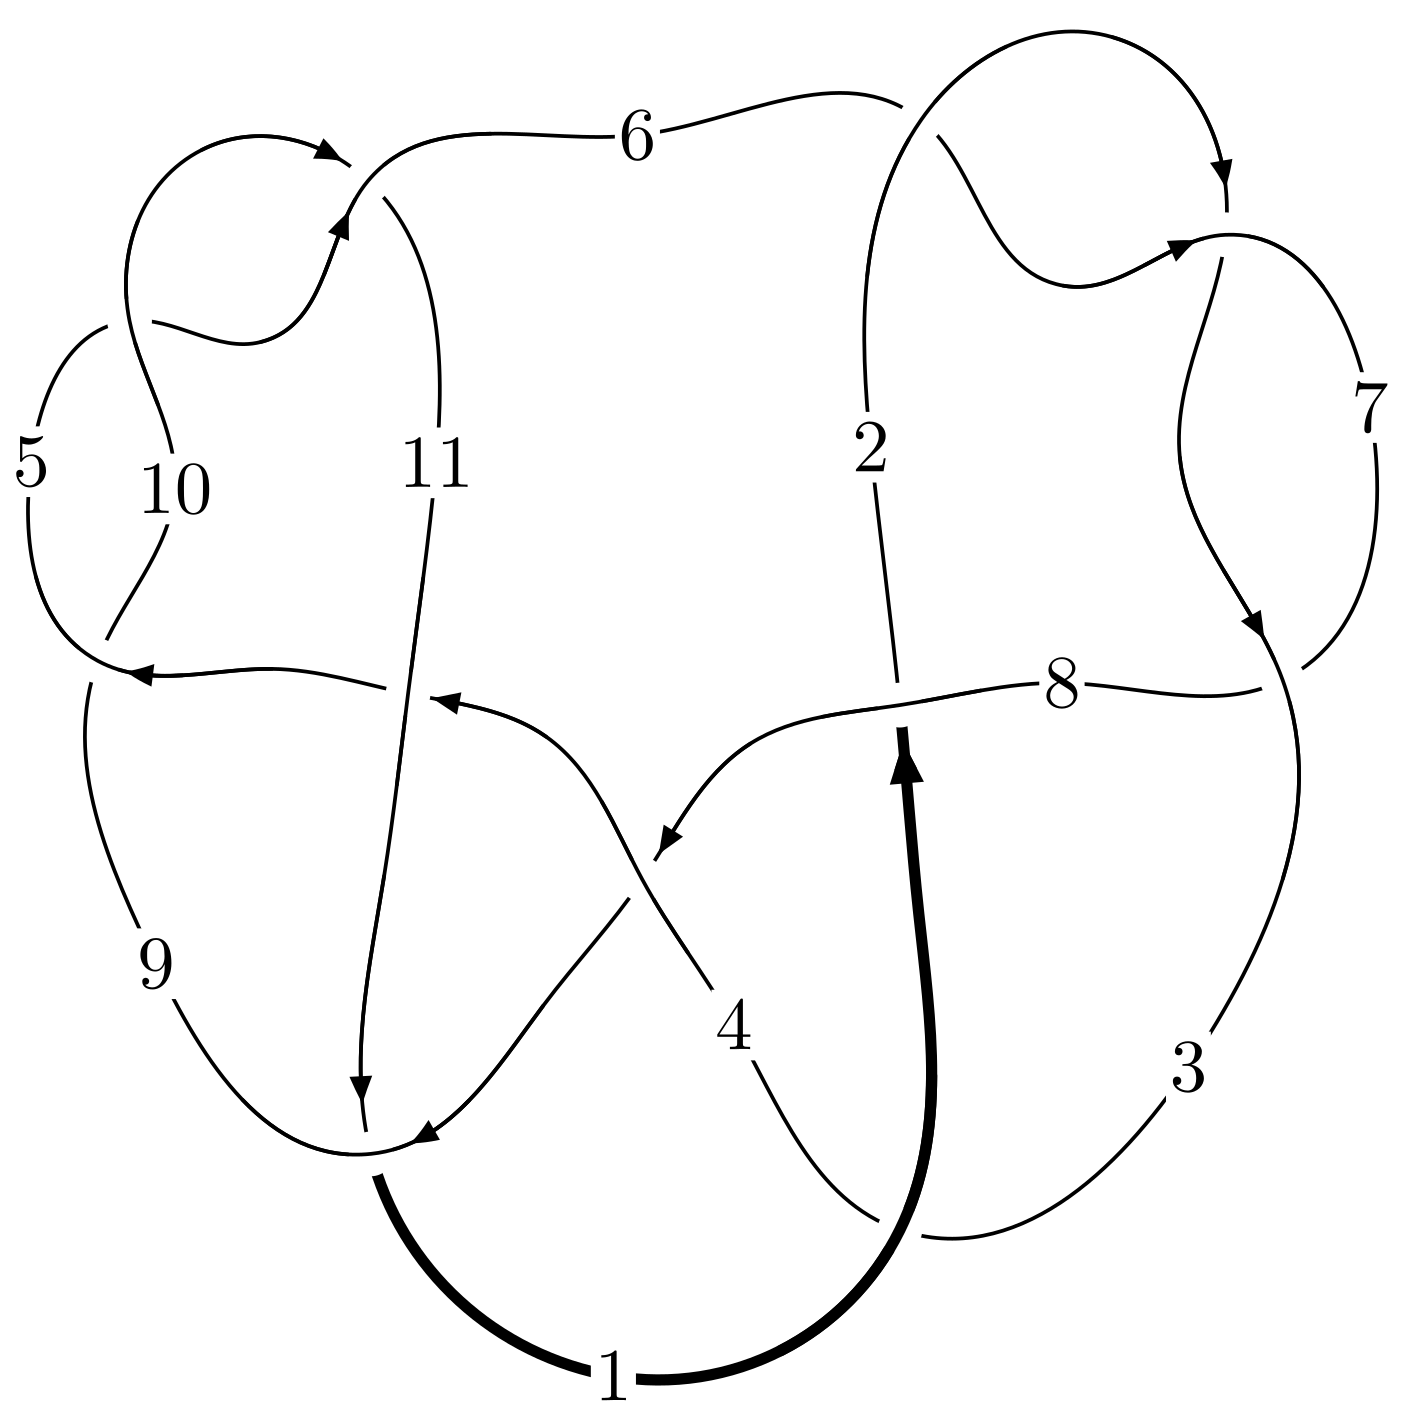
\includegraphics[width=112pt]{../../../GIT/diagram.site/Diagrams/png/555_11a_306.png}\\
\ \ \ A knot diagram\footnotemark}&
\allowdisplaybreaks
\textbf{Linearized knot diagam} \\
\cline{2-2}
 &
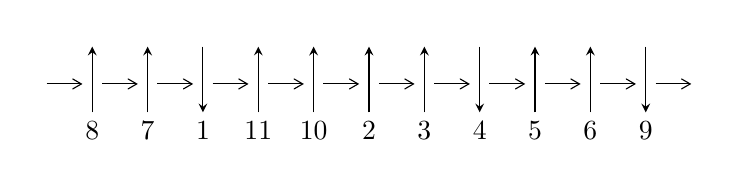
\begin{tikzpicture}[x=20pt, y=17pt]
	% nodes
	\node (C0) at (0, 0) {};
	\node (C1) at (1, 0) {};
	\node (C1U) at (1, +1) {};
	\node (C1D) at (1, -1) {8};

	\node (C2) at (2, 0) {};
	\node (C2U) at (2, +1) {};
	\node (C2D) at (2, -1) {7};

	\node (C3) at (3, 0) {};
	\node (C3U) at (3, +1) {};
	\node (C3D) at (3, -1) {1};

	\node (C4) at (4, 0) {};
	\node (C4U) at (4, +1) {};
	\node (C4D) at (4, -1) {11};

	\node (C5) at (5, 0) {};
	\node (C5U) at (5, +1) {};
	\node (C5D) at (5, -1) {10};

	\node (C6) at (6, 0) {};
	\node (C6U) at (6, +1) {};
	\node (C6D) at (6, -1) {2};

	\node (C7) at (7, 0) {};
	\node (C7U) at (7, +1) {};
	\node (C7D) at (7, -1) {3};

	\node (C8) at (8, 0) {};
	\node (C8U) at (8, +1) {};
	\node (C8D) at (8, -1) {4};

	\node (C9) at (9, 0) {};
	\node (C9U) at (9, +1) {};
	\node (C9D) at (9, -1) {5};

	\node (C10) at (10, 0) {};
	\node (C10U) at (10, +1) {};
	\node (C10D) at (10, -1) {6};

	\node (C11) at (11, 0) {};
	\node (C11U) at (11, +1) {};
	\node (C11D) at (11, -1) {9};
	\node (C12) at (12, 0) {};

	% arrows
	\draw[->,>={angle 60}]
	(C0) edge (C1) (C1) edge (C2) (C2) edge (C3) (C3) edge (C4) (C4) edge (C5) (C5) edge (C6) (C6) edge (C7) (C7) edge (C8) (C8) edge (C9) (C9) edge (C10) (C10) edge (C11) (C11) edge (C12) ;	\draw[->,>=stealth]
	(C1D) edge (C1U) (C2D) edge (C2U) (C3U) edge (C3D) (C4D) edge (C4U) (C5D) edge (C5U) (C6D) edge (C6U) (C7D) edge (C7U) (C8U) edge (C8D) (C9D) edge (C9U) (C10D) edge (C10U) (C11U) edge (C11D) ;
	\end{tikzpicture} \\
\hhline{~~} \\& 
\textbf{Solving Sequence} \\ \cline{2-2} 
 &
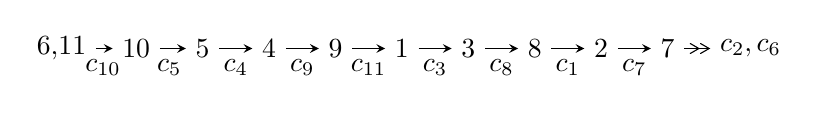
\begin{tikzpicture}[x=24pt, y=7pt]
	% node
	\node (A0) at (-1/8, 0) {6,11};
	\node (A1) at (1, 0) {10};
	\node (A2) at (2, 0) {5};
	\node (A3) at (3, 0) {4};
	\node (A4) at (4, 0) {9};
	\node (A5) at (5, 0) {1};
	\node (A6) at (6, 0) {3};
	\node (A7) at (7, 0) {8};
	\node (A8) at (8, 0) {2};
	\node (A9) at (9, 0) {7};
	\node (C1) at (1/2, -1) {$c_{10}$};
	\node (C2) at (3/2, -1) {$c_{5}$};
	\node (C3) at (5/2, -1) {$c_{4}$};
	\node (C4) at (7/2, -1) {$c_{9}$};
	\node (C5) at (9/2, -1) {$c_{11}$};
	\node (C6) at (11/2, -1) {$c_{3}$};
	\node (C7) at (13/2, -1) {$c_{8}$};
	\node (C8) at (15/2, -1) {$c_{1}$};
	\node (C9) at (17/2, -1) {$c_{7}$};
	\node (A10) at (41/4, 0) {$c_{2},c_{6}$};

	% edge
	\draw[->,>=stealth]	
	(A0) edge (A1) (A1) edge (A2) (A2) edge (A3) (A3) edge (A4) (A4) edge (A5) (A5) edge (A6) (A6) edge (A7) (A7) edge (A8) (A8) edge (A9) ;
	\draw[->>,>={angle 60}]	
	(A9) edge (A10);
\end{tikzpicture} \\ 

\end{tabular} \\

\footnotetext{
The image of knot diagram is generated by the software ``\textbf{Draw programme}" developed by Andrew Bartholomew(\url{http://www.layer8.co.uk/maths/draw/index.htm\#Running-draw}), where we modified some parts for our purpose(\url{https://github.com/CATsTAILs/LinksPainter}).
}\phantom \\ \newline 
\centering \textbf{Ideals for irreducible components\footnotemark of $X_{\text{par}}$} 
 
\begin{align*}
I^u_{1}&=\langle 
u^9+u^8-4 u^7-4 u^6+4 u^5+4 u^4+u^3- u+1\rangle \\
I^u_{2}&=\langle 
u^{42}+u^{41}+\cdots-2 u^4+1\rangle \\
I^u_{3}&=\langle 
u-1\rangle \\
\\
\end{align*}
\raggedright * 3 irreducible components of $\dim_{\mathbb{C}}=0$, with total 52 representations.\\
\footnotetext{All coefficients of polynomials are rational numbers. But the coefficients are sometimes approximated in decimal forms when there is not enough margin.}
\newpage
\renewcommand{\arraystretch}{1}
\centering \section*{I. $I^u_{1}= \langle u^9+u^8-4 u^7-4 u^6+4 u^5+4 u^4+u^3- u+1 \rangle$}
\flushleft \textbf{(i) Arc colorings}\\
\begin{tabular}{m{7pt} m{180pt} m{7pt} m{180pt} }
\flushright $a_{6}=$&$\begin{pmatrix}0\\u\end{pmatrix}$ \\
\flushright $a_{11}=$&$\begin{pmatrix}1\\0\end{pmatrix}$ \\
\flushright $a_{10}=$&$\begin{pmatrix}1\\u^2\end{pmatrix}$ \\
\flushright $a_{5}=$&$\begin{pmatrix}- u\\- u^3+u\end{pmatrix}$ \\
\flushright $a_{4}=$&$\begin{pmatrix}u^3-2 u\\- u^3+u\end{pmatrix}$ \\
\flushright $a_{9}=$&$\begin{pmatrix}- u^2+1\\- u^4+2 u^2\end{pmatrix}$ \\
\flushright $a_{1}=$&$\begin{pmatrix}u^6-3 u^4+2 u^2+1\\u^8-4 u^6+4 u^4\end{pmatrix}$ \\
\flushright $a_{3}=$&$\begin{pmatrix}u^2-1\\u^8-3 u^6- u^5+2 u^4+2 u^3- u+1\end{pmatrix}$ \\
\flushright $a_{8}=$&$\begin{pmatrix}- u^3+2 u\\u^8-3 u^6+u^4+u^3+2 u^2-2 u+1\end{pmatrix}$ \\
\flushright $a_{2}=$&$\begin{pmatrix}1\\u^6-2 u^4- u^3+u-1\end{pmatrix}$ \\
\flushright $a_{7}=$&$\begin{pmatrix}u\\u^7-2 u^5- u^4+u^2\end{pmatrix}$\\ \flushright $a_{7}=$&$\begin{pmatrix}u\\u^7-2 u^5- u^4+u^2\end{pmatrix}$\\&\end{tabular}
\flushleft \textbf{(ii) Obstruction class $= -1$}\\~\\
\flushleft \textbf{(iii) Cusp Shapes $= -4 u^7-4 u^6+16 u^5+12 u^4-16 u^3-8 u^2+10$}\\~\\
\newpage\renewcommand{\arraystretch}{1}
\flushleft \textbf{(iv) u-Polynomials at the component}\newline \\
\begin{tabular}{m{50pt}|m{274pt}}
Crossings & \hspace{64pt}u-Polynomials at each crossing \\
\hline $$\begin{aligned}c_{1},c_{4}\end{aligned}$$&$\begin{aligned}
&u^9- u^7+2 u^6+8 u^5-5 u^4-5 u^3-5 u^2+9 u-3
\end{aligned}$\\
\hline $$\begin{aligned}c_{2},c_{5},c_{6}\\c_{7},c_{9},c_{10}\end{aligned}$$&$\begin{aligned}
&u^9+u^8-4 u^7-4 u^6+4 u^5+4 u^4+u^3- u+1
\end{aligned}$\\
\hline $$\begin{aligned}c_{3},c_{11}\end{aligned}$$&$\begin{aligned}
&u^9- u^8+4 u^7-2 u^6+8 u^5-6 u^4+9 u^3-6 u^2+3 u-1
\end{aligned}$\\
\hline $$\begin{aligned}c_{8}\end{aligned}$$&$\begin{aligned}
&u^9-6 u^8+18 u^7-33 u^6+39 u^5-23 u^4-7 u^3+26 u^2-20 u+8
\end{aligned}$\\
\hline
\end{tabular}\\~\\
\newpage\renewcommand{\arraystretch}{1}
\flushleft \textbf{(v) Riley Polynomials at the component}\newline \\
\begin{tabular}{m{50pt}|m{274pt}}
Crossings & \hspace{64pt}Riley Polynomials at each crossing \\
\hline $$\begin{aligned}c_{1},c_{4}\end{aligned}$$&$\begin{aligned}
&y^9-2 y^8+17 y^7-30 y^6+112 y^5-103 y^4+131 y^3-145 y^2+51 y-9
\end{aligned}$\\
\hline $$\begin{aligned}c_{2},c_{5},c_{6}\\c_{7},c_{9},c_{10}\end{aligned}$$&$\begin{aligned}
&y^9-9 y^8+32 y^7-54 y^6+38 y^5-2 y^4+y^3-10 y^2+y-1
\end{aligned}$\\
\hline $$\begin{aligned}c_{3},c_{11}\end{aligned}$$&$\begin{aligned}
&y^9+7 y^8+28 y^7+66 y^6+106 y^5+106 y^4+53 y^3+6 y^2-3 y-1
\end{aligned}$\\
\hline $$\begin{aligned}c_{8}\end{aligned}$$&$\begin{aligned}
&y^9+6 y^7+25 y^6+23 y^5+17 y^4+213 y^3-28 y^2-16 y-64
\end{aligned}$\\
\hline
\end{tabular}\\~\\
\newpage\flushleft \textbf{(vi) Complex Volumes and Cusp Shapes}
$$\begin{array}{c|c|c}  
\text{Solutions to }I^u_{1}& \I (\text{vol} + \sqrt{-1}CS) & \text{Cusp shape}\\
 \hline 
\begin{aligned}
u &= -0.287064 + 0.695105 I\end{aligned}
 & -1.39752 - 6.41727 I & \phantom{-}2.65899 + 8.21479 I \\ \hline\begin{aligned}
u &= -0.287064 - 0.695105 I\end{aligned}
 & -1.39752 + 6.41727 I & \phantom{-}2.65899 - 8.21479 I \\ \hline\begin{aligned}
u &= -1.30640\phantom{ +0.000000I}\end{aligned}
 & \phantom{-}7.01397\phantom{ +0.000000I} & \phantom{-}12.1820\phantom{ +0.000000I} \\ \hline\begin{aligned}
u &= \phantom{-}0.423257 + 0.356395 I\end{aligned}
 & \phantom{-}0.980950 + 0.551491 I & \phantom{-}9.15793 - 4.50455 I \\ \hline\begin{aligned}
u &= \phantom{-}0.423257 - 0.356395 I\end{aligned}
 & \phantom{-}0.980950 - 0.551491 I & \phantom{-}9.15793 + 4.50455 I \\ \hline\begin{aligned}
u &= -1.42328 + 0.27641 I\end{aligned}
 & \phantom{-}9.5593 - 13.5238 I & \phantom{-}11.6511 + 8.3193 I \\ \hline\begin{aligned}
u &= -1.42328 - 0.27641 I\end{aligned}
 & \phantom{-}9.5593 + 13.5238 I & \phantom{-}11.6511 - 8.3193 I \\ \hline\begin{aligned}
u &= \phantom{-}1.44029 + 0.16872 I\end{aligned}
 & \phantom{-}12.84680 + 4.88120 I & \phantom{-}15.4409 - 3.5107 I \\ \hline\begin{aligned}
u &= \phantom{-}1.44029 - 0.16872 I\end{aligned}
 & \phantom{-}12.84680 - 4.88120 I & \phantom{-}15.4409 + 3.5107 I\\
 \hline 
 \end{array}$$\newpage\newpage\renewcommand{\arraystretch}{1}
\centering \section*{II. $I^u_{2}= \langle u^{42}+u^{41}+\cdots-2 u^4+1 \rangle$}
\flushleft \textbf{(i) Arc colorings}\\
\begin{tabular}{m{7pt} m{180pt} m{7pt} m{180pt} }
\flushright $a_{6}=$&$\begin{pmatrix}0\\u\end{pmatrix}$ \\
\flushright $a_{11}=$&$\begin{pmatrix}1\\0\end{pmatrix}$ \\
\flushright $a_{10}=$&$\begin{pmatrix}1\\u^2\end{pmatrix}$ \\
\flushright $a_{5}=$&$\begin{pmatrix}- u\\- u^3+u\end{pmatrix}$ \\
\flushright $a_{4}=$&$\begin{pmatrix}u^3-2 u\\- u^3+u\end{pmatrix}$ \\
\flushright $a_{9}=$&$\begin{pmatrix}- u^2+1\\- u^4+2 u^2\end{pmatrix}$ \\
\flushright $a_{1}=$&$\begin{pmatrix}u^6-3 u^4+2 u^2+1\\u^8-4 u^6+4 u^4\end{pmatrix}$ \\
\flushright $a_{3}=$&$\begin{pmatrix}- u^{17}+8 u^{15}-25 u^{13}+36 u^{11}-19 u^9-4 u^7+2 u^5+4 u^3- u\\- u^{19}+9 u^{17}-32 u^{15}+55 u^{13}-43 u^{11}+9 u^9+4 u^5- u^3+u\end{pmatrix}$ \\
\flushright $a_{8}=$&$\begin{pmatrix}- u^{10}+5 u^8-8 u^6+3 u^4+u^2+1\\u^{10}-4 u^8+5 u^6-2 u^4+u^2\end{pmatrix}$ \\
\flushright $a_{2}=$&$\begin{pmatrix}u^{28}-13 u^{26}+\cdots+u^2+1\\- u^{28}+12 u^{26}+\cdots+2 u^6+3 u^4\end{pmatrix}$ \\
\flushright $a_{7}=$&$\begin{pmatrix}- u^{41}- u^{40}+\cdots+u+2\\u^{41}-19 u^{39}+\cdots+u-1\end{pmatrix}$\\ \flushright $a_{7}=$&$\begin{pmatrix}- u^{41}- u^{40}+\cdots+u+2\\u^{41}-19 u^{39}+\cdots+u-1\end{pmatrix}$\\&\end{tabular}
\flushleft \textbf{(ii) Obstruction class $= -1$}\\~\\
\flushleft \textbf{(iii) Cusp Shapes $= -4 u^{40}+72 u^{38}-588 u^{36}+2864 u^{34}-4 u^{33}-9192 u^{32}+60 u^{31}+20240 u^{30}-404 u^{29}-30780 u^{28}+1600 u^{27}+31580 u^{26}-4096 u^{25}-20524 u^{24}+6988 u^{23}+7548 u^{22}-7832 u^{21}-1876 u^{20}+5336 u^{19}+1340 u^{18}-1704 u^{17}-664 u^{16}-16 u^{15}-192 u^{14}-116 u^{13}+212 u^{12}+256 u^{11}-28 u^{10}-24 u^9-44 u^8-56 u^7+28 u^6+8 u^5+8 u^4+12 u^3+4 u^2-8 u+6$}\\~\\
\newpage\renewcommand{\arraystretch}{1}
\flushleft \textbf{(iv) u-Polynomials at the component}\newline \\
\begin{tabular}{m{50pt}|m{274pt}}
Crossings & \hspace{64pt}u-Polynomials at each crossing \\
\hline $$\begin{aligned}c_{1},c_{4}\end{aligned}$$&$\begin{aligned}
&u^{42}-3 u^{41}+\cdots-2 u-1
\end{aligned}$\\
\hline $$\begin{aligned}c_{2},c_{5},c_{6}\\c_{7},c_{9},c_{10}\end{aligned}$$&$\begin{aligned}
&u^{42}+u^{41}+\cdots-2 u^4+1
\end{aligned}$\\
\hline $$\begin{aligned}c_{3},c_{11}\end{aligned}$$&$\begin{aligned}
&u^{42}-9 u^{41}+\cdots-920 u+113
\end{aligned}$\\
\hline $$\begin{aligned}c_{8}\end{aligned}$$&$\begin{aligned}
&(u^{21}+3 u^{20}+\cdots+4 u-1)^{2}
\end{aligned}$\\
\hline
\end{tabular}\\~\\
\newpage\renewcommand{\arraystretch}{1}
\flushleft \textbf{(v) Riley Polynomials at the component}\newline \\
\begin{tabular}{m{50pt}|m{274pt}}
Crossings & \hspace{64pt}Riley Polynomials at each crossing \\
\hline $$\begin{aligned}c_{1},c_{4}\end{aligned}$$&$\begin{aligned}
&y^{42}- y^{41}+\cdots-24 y+1
\end{aligned}$\\
\hline $$\begin{aligned}c_{2},c_{5},c_{6}\\c_{7},c_{9},c_{10}\end{aligned}$$&$\begin{aligned}
&y^{42}-37 y^{41}+\cdots-4 y^2+1
\end{aligned}$\\
\hline $$\begin{aligned}c_{3},c_{11}\end{aligned}$$&$\begin{aligned}
&y^{42}+11 y^{41}+\cdots+84720 y+12769
\end{aligned}$\\
\hline $$\begin{aligned}c_{8}\end{aligned}$$&$\begin{aligned}
&(y^{21}-3 y^{20}+\cdots+52 y-1)^{2}
\end{aligned}$\\
\hline
\end{tabular}\\~\\
\newpage\flushleft \textbf{(vi) Complex Volumes and Cusp Shapes}
$$\begin{array}{c|c|c}  
\text{Solutions to }I^u_{2}& \I (\text{vol} + \sqrt{-1}CS) & \text{Cusp shape}\\
 \hline 
\begin{aligned}
u &= \phantom{-}1.08927\phantom{ +0.000000I}\end{aligned}
 & \phantom{-}1.57667\phantom{ +0.000000I} & \phantom{-}7.15490\phantom{ +0.000000I} \\ \hline\begin{aligned}
u &= -1.082920 + 0.161904 I\end{aligned}
 & -0.40568 - 3.16875 I & \phantom{-}2.95224 + 5.22442 I \\ \hline\begin{aligned}
u &= -1.082920 - 0.161904 I\end{aligned}
 & -0.40568 + 3.16875 I & \phantom{-}2.95224 - 5.22442 I \\ \hline\begin{aligned}
u &= \phantom{-}1.112720 + 0.206888 I\end{aligned}
 & \phantom{-}4.64745 + 6.55351 I & \phantom{-}8.17560 - 6.03047 I \\ \hline\begin{aligned}
u &= \phantom{-}1.112720 - 0.206888 I\end{aligned}
 & \phantom{-}4.64745 - 6.55351 I & \phantom{-}8.17560 + 6.03047 I \\ \hline\begin{aligned}
u &= \phantom{-}0.301718 + 0.707163 I\end{aligned}
 & \phantom{-}4.04389 + 9.94224 I & \phantom{-}7.31059 - 8.24169 I \\ \hline\begin{aligned}
u &= \phantom{-}0.301718 - 0.707163 I\end{aligned}
 & \phantom{-}4.04389 - 9.94224 I & \phantom{-}7.31059 + 8.24169 I \\ \hline\begin{aligned}
u &= \phantom{-}0.619519 + 0.389305 I\end{aligned}
 & \phantom{-}5.30545 - 6.06326 I & \phantom{-}10.03226 + 2.92445 I \\ \hline\begin{aligned}
u &= \phantom{-}0.619519 - 0.389305 I\end{aligned}
 & \phantom{-}5.30545 + 6.06326 I & \phantom{-}10.03226 - 2.92445 I \\ \hline\begin{aligned}
u &= -0.335269 + 0.641117 I\end{aligned}
 & \phantom{-}6.08429 - 1.09840 I & \phantom{-}10.14786 + 3.17531 I \\ \hline\begin{aligned}
u &= -0.335269 - 0.641117 I\end{aligned}
 & \phantom{-}6.08429 + 1.09840 I & \phantom{-}10.14786 - 3.17531 I \\ \hline\begin{aligned}
u &= \phantom{-}0.274697 + 0.655623 I\end{aligned}
 & -0.07785 + 2.71696 I & \phantom{-}5.48517 - 3.12164 I \\ \hline\begin{aligned}
u &= \phantom{-}0.274697 - 0.655623 I\end{aligned}
 & -0.07785 - 2.71696 I & \phantom{-}5.48517 + 3.12164 I \\ \hline\begin{aligned}
u &= \phantom{-}0.211792 + 0.670835 I\end{aligned}
 & -0.40568 + 3.16875 I & \phantom{-}2.95224 - 5.22442 I \\ \hline\begin{aligned}
u &= \phantom{-}0.211792 - 0.670835 I\end{aligned}
 & -0.40568 - 3.16875 I & \phantom{-}2.95224 + 5.22442 I \\ \hline\begin{aligned}
u &= -0.594417 + 0.333320 I\end{aligned}
 & -0.07785 + 2.71696 I & \phantom{-}5.48517 - 3.12164 I \\ \hline\begin{aligned}
u &= -0.594417 - 0.333320 I\end{aligned}
 & -0.07785 - 2.71696 I & \phantom{-}5.48517 + 3.12164 I \\ \hline\begin{aligned}
u &= \phantom{-}0.096884 + 0.668841 I\end{aligned}
 & \phantom{-}1.62697 - 3.23317 I & \phantom{-}3.55215 + 1.92093 I \\ \hline\begin{aligned}
u &= \phantom{-}0.096884 - 0.668841 I\end{aligned}
 & \phantom{-}1.62697 + 3.23317 I & \phantom{-}3.55215 - 1.92093 I \\ \hline\begin{aligned}
u &= -0.481440 + 0.468716 I\end{aligned}
 & \phantom{-}6.75483 - 2.56601 I & \phantom{-}12.00469 + 3.90900 I \\ \hline\begin{aligned}
u &= -0.481440 - 0.468716 I\end{aligned}
 & \phantom{-}6.75483 + 2.56601 I & \phantom{-}12.00469 - 3.90900 I \\ \hline\begin{aligned}
u &= -0.147288 + 0.653126 I\end{aligned}
 & -3.11833\phantom{ +0.000000I} & -1.91795 + 0. I\phantom{ +0.000000I} \\ \hline\begin{aligned}
u &= -0.147288 - 0.653126 I\end{aligned}
 & -3.11833\phantom{ +0.000000I} & -1.91795 + 0. I\phantom{ +0.000000I} \\ \hline\begin{aligned}
u &= -1.317380 + 0.229558 I\end{aligned}
 & \phantom{-}6.02305\phantom{ +0.000000I} & \phantom{-0.000000 } 0 \\ \hline\begin{aligned}
u &= -1.317380 - 0.229558 I\end{aligned}
 & \phantom{-}6.02305\phantom{ +0.000000I} & \phantom{-0.000000 } 0 \\ \hline\begin{aligned}
u &= \phantom{-}0.644973\phantom{ +0.000000I}\end{aligned}
 & \phantom{-}1.57667\phantom{ +0.000000I} & \phantom{-}7.15490\phantom{ +0.000000I} \\ \hline\begin{aligned}
u &= \phantom{-}1.354040 + 0.243767 I\end{aligned}
 & \phantom{-}1.62697 + 3.23317 I & \phantom{-0.000000 } 0 \\ \hline\begin{aligned}
u &= \phantom{-}1.354040 - 0.243767 I\end{aligned}
 & \phantom{-}1.62697 - 3.23317 I & \phantom{-0.000000 } 0 \\ \hline\begin{aligned}
u &= -1.379260 + 0.261235 I\end{aligned}
 & \phantom{-}4.64745 - 6.55351 I & \phantom{-0.000000 } 0 \\ \hline\begin{aligned}
u &= -1.379260 - 0.261235 I\end{aligned}
 & \phantom{-}4.64745 + 6.55351 I & \phantom{-0.000000 } 0\\
 \hline 
 \end{array}$$\newpage$$\begin{array}{c|c|c}  
\text{Solutions to }I^u_{2}& \I (\text{vol} + \sqrt{-1}CS) & \text{Cusp shape}\\
 \hline 
\begin{aligned}
u &= -1.41719 + 0.15750 I\end{aligned}
 & \phantom{-}6.75483 - 2.56601 I & \phantom{-0.000000 } 0 \\ \hline\begin{aligned}
u &= -1.41719 - 0.15750 I\end{aligned}
 & \phantom{-}6.75483 + 2.56601 I & \phantom{-0.000000 } 0 \\ \hline\begin{aligned}
u &= \phantom{-}1.42429 + 0.12838 I\end{aligned}
 & \phantom{-}6.08429 - 1.09840 I & \phantom{-0.000000 } 0 \\ \hline\begin{aligned}
u &= \phantom{-}1.42429 - 0.12838 I\end{aligned}
 & \phantom{-}6.08429 + 1.09840 I & \phantom{-0.000000 } 0 \\ \hline\begin{aligned}
u &= -1.40967 + 0.25849 I\end{aligned}
 & \phantom{-}5.30545 - 6.06326 I & \phantom{-0.000000 } 0 \\ \hline\begin{aligned}
u &= -1.40967 - 0.25849 I\end{aligned}
 & \phantom{-}5.30545 + 6.06326 I & \phantom{-0.000000 } 0 \\ \hline\begin{aligned}
u &= \phantom{-}1.41609 + 0.27243 I\end{aligned}
 & \phantom{-}4.04389 + 9.94224 I & \phantom{-0.000000 } 0 \\ \hline\begin{aligned}
u &= \phantom{-}1.41609 - 0.27243 I\end{aligned}
 & \phantom{-}4.04389 - 9.94224 I & \phantom{-0.000000 } 0 \\ \hline\begin{aligned}
u &= -1.44204 + 0.12357 I\end{aligned}
 & \phantom{-}11.72580 + 4.35170 I & \phantom{-0.000000 } 0 \\ \hline\begin{aligned}
u &= -1.44204 - 0.12357 I\end{aligned}
 & \phantom{-}11.72580 - 4.35170 I & \phantom{-0.000000 } 0 \\ \hline\begin{aligned}
u &= \phantom{-}1.42800 + 0.24722 I\end{aligned}
 & \phantom{-}11.72580 + 4.35170 I & \phantom{-0.000000 } 0 \\ \hline\begin{aligned}
u &= \phantom{-}1.42800 - 0.24722 I\end{aligned}
 & \phantom{-}11.72580 - 4.35170 I & \phantom{-0.000000 } 0\\
 \hline 
 \end{array}$$\newpage\newpage\renewcommand{\arraystretch}{1}
\centering \section*{III. $I^u_{3}= \langle u-1 \rangle$}
\flushleft \textbf{(i) Arc colorings}\\
\begin{tabular}{m{7pt} m{180pt} m{7pt} m{180pt} }
\flushright $a_{6}=$&$\begin{pmatrix}0\\1\end{pmatrix}$ \\
\flushright $a_{11}=$&$\begin{pmatrix}1\\0\end{pmatrix}$ \\
\flushright $a_{10}=$&$\begin{pmatrix}1\\1\end{pmatrix}$ \\
\flushright $a_{5}=$&$\begin{pmatrix}-1\\0\end{pmatrix}$ \\
\flushright $a_{4}=$&$\begin{pmatrix}-1\\0\end{pmatrix}$ \\
\flushright $a_{9}=$&$\begin{pmatrix}0\\1\end{pmatrix}$ \\
\flushright $a_{1}=$&$\begin{pmatrix}1\\1\end{pmatrix}$ \\
\flushright $a_{3}=$&$\begin{pmatrix}0\\1\end{pmatrix}$ \\
\flushright $a_{8}=$&$\begin{pmatrix}1\\1\end{pmatrix}$ \\
\flushright $a_{2}=$&$\begin{pmatrix}1\\1\end{pmatrix}$ \\
\flushright $a_{7}=$&$\begin{pmatrix}1\\2\end{pmatrix}$\\ \flushright $a_{7}=$&$\begin{pmatrix}1\\2\end{pmatrix}$\\&\end{tabular}
\flushleft \textbf{(ii) Obstruction class $= -1$}\\~\\
\flushleft \textbf{(iii) Cusp Shapes $= 6$}\\~\\
\newpage\renewcommand{\arraystretch}{1}
\flushleft \textbf{(iv) u-Polynomials at the component}\newline \\
\begin{tabular}{m{50pt}|m{274pt}}
Crossings & \hspace{64pt}u-Polynomials at each crossing \\
\hline $$\begin{aligned}c_{1},c_{4}\end{aligned}$$&$\begin{aligned}
&u
\end{aligned}$\\
\hline $$\begin{aligned}c_{2},c_{3},c_{5}\\c_{6},c_{7},c_{8}\\c_{9},c_{10},c_{11}\end{aligned}$$&$\begin{aligned}
&u-1
\end{aligned}$\\
\hline
\end{tabular}\\~\\
\newpage\renewcommand{\arraystretch}{1}
\flushleft \textbf{(v) Riley Polynomials at the component}\newline \\
\begin{tabular}{m{50pt}|m{274pt}}
Crossings & \hspace{64pt}Riley Polynomials at each crossing \\
\hline $$\begin{aligned}c_{1},c_{4}\end{aligned}$$&$\begin{aligned}
&y
\end{aligned}$\\
\hline $$\begin{aligned}c_{2},c_{3},c_{5}\\c_{6},c_{7},c_{8}\\c_{9},c_{10},c_{11}\end{aligned}$$&$\begin{aligned}
&y-1
\end{aligned}$\\
\hline
\end{tabular}\\~\\
\newpage\flushleft \textbf{(vi) Complex Volumes and Cusp Shapes}
$$\begin{array}{c|c|c}  
\text{Solutions to }I^u_{3}& \I (\text{vol} + \sqrt{-1}CS) & \text{Cusp shape}\\
 \hline 
\begin{aligned}
u &= \phantom{-}1.00000\phantom{ +0.000000I}\end{aligned}
 & \phantom{-}1.64493\phantom{ +0.000000I} & \phantom{-}6.00000\phantom{ +0.000000I}\\
 \hline 
 \end{array}$$\newpage
\newpage\renewcommand{\arraystretch}{1}
\centering \section*{ IV. u-Polynomials}
\begin{tabular}{m{50pt}|m{274pt}}
Crossings & \hspace{64pt}u-Polynomials at each crossing \\
\hline $$\begin{aligned}c_{1},c_{4}\end{aligned}$$&$\begin{aligned}
&u(u^9- u^7+2 u^6+8 u^5-5 u^4-5 u^3-5 u^2+9 u-3)\\
&\cdot(u^{42}-3 u^{41}+\cdots-2 u-1)
\end{aligned}$\\
\hline $$\begin{aligned}c_{2},c_{5},c_{6}\\c_{7},c_{9},c_{10}\end{aligned}$$&$\begin{aligned}
&(u-1)(u^9+u^8-4 u^7-4 u^6+4 u^5+4 u^4+u^3- u+1)\\
&\cdot(u^{42}+u^{41}+\cdots-2 u^4+1)
\end{aligned}$\\
\hline $$\begin{aligned}c_{3},c_{11}\end{aligned}$$&$\begin{aligned}
&(u-1)(u^9- u^8+4 u^7-2 u^6+8 u^5-6 u^4+9 u^3-6 u^2+3 u-1)\\
&\cdot(u^{42}-9 u^{41}+\cdots-920 u+113)
\end{aligned}$\\
\hline $$\begin{aligned}c_{8}\end{aligned}$$&$\begin{aligned}
&(u-1)(u^9-6 u^8+\cdots-20 u+8)\\
&\cdot(u^{21}+3 u^{20}+\cdots+4 u-1)^{2}
\end{aligned}$\\
\hline
\end{tabular}\newpage\renewcommand{\arraystretch}{1}
\centering \section*{ V. Riley Polynomials}
\begin{tabular}{m{50pt}|m{274pt}}
Crossings & \hspace{64pt}Riley Polynomials at each crossing \\
\hline $$\begin{aligned}c_{1},c_{4}\end{aligned}$$&$\begin{aligned}
&y\\
&\cdot(y^9-2 y^8+17 y^7-30 y^6+112 y^5-103 y^4+131 y^3-145 y^2+51 y-9)\\
&\cdot(y^{42}- y^{41}+\cdots-24 y+1)
\end{aligned}$\\
\hline $$\begin{aligned}c_{2},c_{5},c_{6}\\c_{7},c_{9},c_{10}\end{aligned}$$&$\begin{aligned}
&(y-1)(y^9-9 y^8+32 y^7-54 y^6+38 y^5-2 y^4+y^3-10 y^2+y-1)\\
&\cdot(y^{42}-37 y^{41}+\cdots-4 y^2+1)
\end{aligned}$\\
\hline $$\begin{aligned}c_{3},c_{11}\end{aligned}$$&$\begin{aligned}
&(y-1)(y^9+7 y^8+\cdots-3 y-1)\\
&\cdot(y^{42}+11 y^{41}+\cdots+84720 y+12769)
\end{aligned}$\\
\hline $$\begin{aligned}c_{8}\end{aligned}$$&$\begin{aligned}
&(y-1)(y^9+6 y^7+\cdots-16 y-64)\\
&\cdot(y^{21}-3 y^{20}+\cdots+52 y-1)^{2}
\end{aligned}$\\
\hline
\end{tabular}
\vskip 2pc
\end{document}